\chapter{Pseudoinverses and the SVD}

\section{Singular Value Decomposition}

Singular Value Decomposition is a fundamental technique in Linear Algebra, particularly for dealing with non-square matrices.

\subsection{Diagonalization of a Matrix}
Consider a matrix \( A \) of dimension \( m \times n \) and rank \( r \). To diagonalize \( A \), we usually perform a transformation \( A = S\Lambda S^{-1} \). However, this approach has limitations:
\begin{itemize}
    \item The matrix \( A \) must be square.
    \item There may not be a sufficient number of eigenvectors to form the matrix \( S \).
\end{itemize}

For example, the matrix 
\( \begin{pmatrix}
1 & a \\
0 & 1
\end{pmatrix} \)
with \( a \neq 0 \) has only the eigenvector \( \begin{pmatrix} x & 0 \end{pmatrix} \).

\textbf{Goal:} We seek a type of decomposition that applies to any matrix.

\subsection{The Singular Value Decomposition Theorem}

\textbf{Theorem:}

Every matrix \( A \in \mathbb{C}^{m \times n} \) can be factored as \( A = U\Sigma V^H \), where:
\begin{itemize}
    \item \( U \) is a unitary matrix \( (U^H U = I) \) with columns \( u_i \) and dimension \( m \times m \).
    \item \( \Sigma \) is an \( m \times n \) rectangular matrix with non-negative real entries along the main diagonal.
    \item \( V \) is a unitary matrix \( (V^H V = I) \) with columns \( v_i \) and dimension \( n \times n \).
\end{itemize}


\begin{itemize}
    \item \( U \) is generally different from \( V \).
    \item The elements of \( \Sigma \), called the singular values of \( A \), are positive and typically ordered.
    \item For square invertible matrices, this decomposition is similar to the eigendecomposition.
\end{itemize}

\subsection{Properties of SVD}
\begin{itemize}
    \item If \( m = 2 \) and \( n = 3 \), \( \Sigma \) would look like \( \begin{pmatrix} \sigma_1 & 0 & 0 \\ 0 & \sigma_2 & 0 \end{pmatrix} \).
    \item \( A^H A = V\Sigma^T U^H U\Sigma V^H = V\Sigma^T \Sigma V^H \), indicating \( \sigma_i^2 \) are the eigenvalues of \( A^H A \) and \( V \) contains the eigenvectors.
    \item Similarly, \( AA^H = U\Sigma V^H V\Sigma^T U^H = U\Sigma \Sigma^T U^H \), showing \( \sigma_i^2 \) are the eigenvalues of \( AA^H \) and \( U \) contains the eigenvectors.
    \item The non-zero elements of \( \Sigma \Sigma^T \) and \( \Sigma^T \Sigma \) are identical.
\end{itemize}

% \textbf{Conclusion:} SVD allows us to decompose any matrix into a product of three matrices, capturing the essence of the matrix in terms of its singular values and vectors.

\subsection{More properties of the SVD}

Matrices \( A \), \( A^H A \) and \( AA^H \) have the same rank.

Let \( A \) be an \( m \times n \) matrix with rank \( r \). The matrix \( A \) has \( r \) singular values. Both \( A^H A \) and \( AA^H \) have \( r \) non-zero eigenvalues which are the squares of the singular values of \( A \). Furthermore:
\begin{itemize}
    \item \( A^H A \) is of dimension \( n \times n \). It has \( r \) eigenvectors \( \{v_1, \ldots, v_r\} \) associated with its \( r \) non-zero eigenvalues and \( n - r \) eigenvectors associated with its \( n - r \) zero eigenvalues.
    \item \( AA^H \) is of dimension \( m \times m \). It has \( r \) eigenvectors \( \{u_1, \ldots, u_r\} \) associated with its \( r \) non-zero eigenvalues and \( m - r \) eigenvectors associated with its \( m - r \) zero eigenvalues.
\end{itemize}

We can write \( V = [v_1 \ldots v_r v_{r+1} \ldots v_n] \) and \( U = [u_1 \ldots u_r u_{r+1} \ldots u_m] \).\\

Note that in the above matrices, we put first in the columns the eigenvectors of \( A^H A \) and \( AA^H \) which correspond to non-zero eigenvalues. We usually order the eigenvectors according to the magnitude of the associated eigenvalue, so the eigenvector that corresponds to the maximum eigenvalue is placed in the first column and so on.\\


As already shown, from \( A = U\Sigma V^H \) we obtain that \( AV = U\Sigma \) or \( A[v_1 \ldots v_r v_{r+1} \ldots v_n] = [u_1 \ldots u_r u_{r+1} \ldots u_m]\Sigma \).\\

Therefore, we can break \( AV = U\Sigma \) into a set of relationships of the form \( Av_i = \sigma_i u_i \). Note that \( \sigma_i \) is a scalar and \( v_i \) and \( u_i \) vectors.\\

For \( i \leq r \) the relationship \( AV = U\Sigma \) tells us that:
\begin{itemize}
    \item The vectors \( u_1, u_2, \ldots, u_r \) are in the column space of \( A \). This observation comes directly from \( u_i = \frac{1}{\sigma_i} Av_i, \sigma_i \neq 0 \), i.e., \( u_i \)s are linear combinations of columns of \( A \). Furthermore, the \( u_i \)s associated with \( \sigma_i \neq 0 \) are orthonormal. Thus, they form a basis of the column space.
    \item The vectors \( v_1, v_2, \ldots, v_r \) are in the row space of \( A \). This is because from \( AV = U\Sigma \) we have \( U^H AV^H = U^H U\Sigma V^H \) \( \Rightarrow U^H A = \Sigma V^H \) \( \Rightarrow A^H = V\Sigma^H U^H \) \( \Rightarrow A^H = V\bar{\Sigma} U^H \), where \( \bar{\Sigma} \) is \( \Sigma^H \) with non-zero elements \( \frac{1}{\sigma_i} \), \( \sigma_i \neq 0 \). Furthermore, since the \( v_i \)'s associated with \( \sigma_i \neq 0 \) are orthonormal, they form a basis of the row space.

\end{itemize}

\begin{itemize}
    \item $\textbf{Av}_i = \sigma_i \textbf{u}_i$ 
    \item $\textbf{v}^\top_i = \frac{1}{\sigma_i}\textbf{u}^\top_i\textbf{A} $
    \item $\textbf{v}_i$ forms an orthonormal basis for the row space of \textbf{A}
    \item $\textbf{u}_i$ forms an orthonormal basis for the column space of \textbf{A}
    \item Any extra $n - r$ additional \textbf{v}'s corresponding to zero eigenvalues of $\textbf{A}^H\textbf{A}$ are taken from the null space of \textbf{A}.
    \item Any extra $m - r$ additional \textbf{u}'s corresponding to zero eigenvalues of $\textbf{A}\textbf{A}^H$ are taken from the null space of $\textbf{A}^H$.
\end{itemize}

We split \( [v_1 \quad \ldots \quad v_r \quad v_{r+1} \quad \ldots \quad v_n] = [V_1 \quad V_2] \) and \( [u_1 \quad \ldots \quad u_r \quad u_{r+1} \quad \ldots \quad u_m] = [U_1 \quad U_2] \), it then follows that:

\[A\begin{bmatrix}v_1&...&v_r & v_{r+1} & ...& v_n\end{bmatrix}=\begin{bmatrix}u_1&...&u_r& u_{r+1} & ...& u_m\end{bmatrix}\Sigma\]


\begin{itemize}
    \item \( \mathcal{R}(A) = \text{span}\{U_1\} \),
    \item \( \mathcal{N}(A) = \text{span}\{V_2\} \),
    \item \( \mathcal{R}(A^H) = \text{span}\{V_1\} \),
    \item \( \mathcal{N}(A^H) = \text{span}\{U_2\} \).
\end{itemize}

\begin{definitionbox}{Truncated or Reduced Singular Value Decomposition}
We can visualise the $AV = U\Sigma$ as such, ignoring eigenvectors that correspond to zero eigenvalues, making $\Sigma$ a square matrix:
\[A\begin{bmatrix}v_1&...&v_r\end{bmatrix}=\begin{bmatrix}u_1&...&u_r\end{bmatrix}\begin{bmatrix}\sigma_1&\cdots&0\\\vdots&\ddots&\vdots\\0&\cdots&\sigma_r\end{bmatrix}\Rightarrow A=u_1\sigma_1v_1^H+\cdots+u_r\sigma_rv_r^H = A=\sum_{i=1}^r\sigma_i\boldsymbol{u}_i\boldsymbol{v}_i^H\]

\begin{itemize}
    \item The dimension of \( A \) is \( m \times n \).
    \item The dimension of \( [v_1 \quad \ldots \quad v_r] \) is \( n \times r \).
    \item The dimension of \( [u_1 \quad \ldots \quad u_r] \) is \( m \times r \).
    \item The dimension of \( \Sigma \) is \( r \times r \).
\end{itemize}

Which is the form for the Truncated or Reduced Singular Value Decomposition, which is the sum of r rank-one matrices.

\end{definitionbox}


\section{Relating the SVD to the pseudo-inverse}

We now go back to the solution to \( A\mathbf{x} = \mathbf{b} \) when \( A \) is neither full column nor row rank.\\

\textbf{Claim:} The Minimum Norm Least Squares solution to \( A\mathbf{x} = \mathbf{b} \) is given by \( \mathbf{x} = A^+\mathbf{b} \) where \( A^+ \) is the pseudoinverse of \( A = U\Sigma V^H \) and is given by \( A^+ = V\Sigma^+U^H \) where\\

\[\mathbf{\Sigma}^{+}=\begin{pmatrix}\frac{1}{\sigma_{1}}&&&&&\\&\ddots&&&&\\&&\frac{1}{\sigma_{r}}&&&\\&&&0&&\\&&&&&\ddots\end{pmatrix}\]

\textbf{Proof:}
We rewrite our problem as:
\[
\min_{\mathbf{x}} \|A\mathbf{x} - \mathbf{b}\| = \min_{\mathbf{x}} \|U\Sigma V^H\mathbf{x} - \mathbf{b}\| = \min_{\mathbf{x}} \| \Sigma V^H\mathbf{x} - U^H\mathbf{b} \|
\]
where the last equality follows from the fact that \( U \) is unitary.

We denote with \( \mathbf{v} = V^H\mathbf{x} \) and \( \mathbf{\tilde{b}} = U^H\mathbf{b} \) then the least-squares problem reduces to 
\[
\min_{\mathbf{v}} \|\Sigma\mathbf{v} - \mathbf{\tilde{b}}\|
\]
for which we know the solution is \( \mathbf{v} = \Sigma^+\mathbf{\tilde{b}} \).

By working backwards we then find the MNLS solution

\[ V^H\mathbf{\hat{x}} = \Sigma^+U^H\mathbf{b}\]\[\Rightarrow \mathbf{\hat{x}} = V\Sigma^+U^H\mathbf{b} \].

\section{Applications of the SVD}
\subsection{Low Rank Approximation}

Given a matrix \( D \), the goal of a low-rank approximation is to find a matrix \( \tilde{D} \) with rank \( r \) that approximates \( D \). This is particularly useful when \( D \) is noisy, or we know a priori that \( D \) is rank deficient.

\subsubsection*{Frobenius Norm}

To measure the approximation, we use the Frobenius norm. For a matrix \( A \), it is defined as:
\[
\|A\|_F = \left( \sum_{i,j} |a_{i,j}|^2 \right)^{\frac{1}{2}} = \left( \text{trace}(A^HA) \right)^{\frac{1}{2}} = \left( \sum_{i} \sigma_i^2 \right)^{\frac{1}{2}}
\]
where \( \sigma_i \) are the singular values of \( A \).

\subsubsection*{Singular Value Decomposition (SVD)}

The Singular Value Decomposition of \( D \) is given by \( D = U\Sigma V^H \), where \( U \) and \( V \) are unitary matrices, \( \Sigma \) is a diagonal matrix with non-negative real numbers on the diagonal (the singular values), and \( H \) denotes the conjugate transpose.

\subsubsection*{Rank-\( r \) Approximation}

For a rank-\( r \) approximation, we consider:
\[
\tilde{D} = \sum_{i=1}^r \sigma_i u_i v_i^H
\]

We can visualise the \( U\Sigma V^H \) as such, ignoring eigenvectors that correspond to zero eigenvalues, making \( \Sigma \) a square matrix:
\[
D\begin{bmatrix}v_1&\cdots&v_r\end{bmatrix} = \begin{bmatrix}u_1&\cdots&u_r\end{bmatrix}\begin{bmatrix}\sigma_1&\cdots&0\\\vdots&\ddots&\vdots\\0&\cdots&\sigma_r\end{bmatrix} \Rightarrow D = u_1\sigma_1v_1^H + \cdots + u_r\sigma_rv_r^H = \sum_{i=1}^r \sigma_i \bm{u}_i \bm{v}_i^H
\]

\begin{itemize}
    \item The dimension of \( D \) is \( m \times n \).
    \item The dimension of \( [v_1 \quad \cdots \quad v_r] \) is \( n \times r \).
    \item The dimension of \( [u_1 \quad \cdots \quad u_r] \) is \( m \times r \).
    \item The dimension of \( \Sigma \) is \( r \times r \).
\end{itemize}

This is the form for the Truncated or Reduced Singular Value Decomposition, which is the sum of \( r \) rank-one matrices.

\subsection{Principal Component Analysis}
Principal Component Analysis (PCA) is a statistical procedure that uses an orthogonal transformation to convert a set of observations of possibly correlated variables into a set of values of linearly uncorrelated variables called principal components.

\subsubsection*{Data Matrix and Mean Centering}

Consider a data matrix \( X \) with \( n \) columns and \( m \) rows, where the columns represent the number of samples and the rows correspond to \( m \) variables measured for each sample (e.g., height, weight, etc.). The preprocessing step in PCA involves mean centering, where the mean value is removed from each row.

\subsubsection*{Principal Components}

The principal components of the data are selected so that the \( i \)-th principal component is the linear combination of the data that accounts for the \( i \)-th largest portion of the variance of the data.

\subsubsection*{First Principal Component}

The first principal component \( a_1 \) is a linear combination \( y_1^T = a_1^T X \) such that the sample variance of \( y_{1,i} \) is maximised subject to the constraint \( ||a_1|| = 1 \).\\

The sample variance \( \sigma_{y_1}^2 \) is given by:
\[
\sigma_{y_1}^2 = \frac{1}{n-1} \sum_{i=1}^n y_{1,i}^2 = \frac{1}{n-1} \sum_{i=1}^n (a_1^T x_i)^2 = a_1^T S a_1
\]
where \( S \) is the covariance matrix:
\[
S = \frac{1}{n-1} XX^T
\]

Maximising \( a_1^T S a_1 \) subject to \( ||a_1|| = 1 \) leads us to an eigenvalue problem, and the solution is the eigenvector corresponding to the largest eigenvalue of \( S \). This is equivalent to the left singular vector of \( X \) related to its largest singular value.

\subsubsection*{Second Principal Component}

The second principal component \( a_2 \) is chosen so that \( y_2^T = a_2^T X \) is uncorrelated with \( y_1 \), which leads to the constraint \( a_2^T a_1 = 0 \). This vector is the singular vector related to the second largest singular value of \( X \).


\begin{figure}[H]
    \centering
    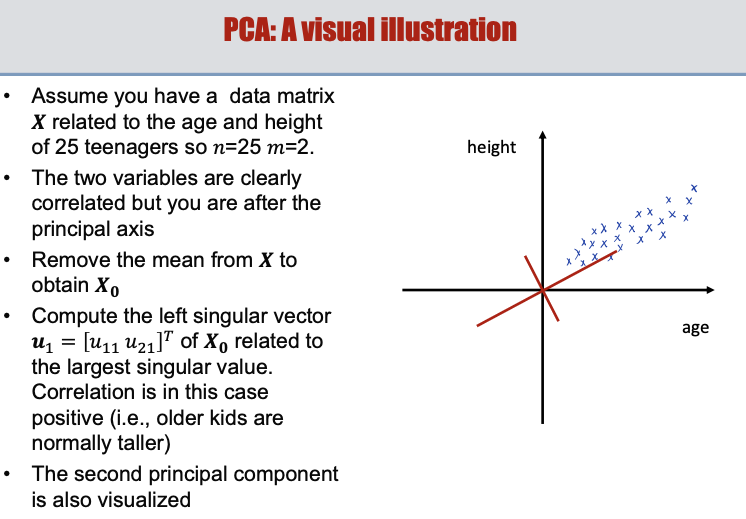
\includegraphics[width=0.75\linewidth]{img/pca-eg.png}
    
    
\end{figure}
\subsection{Total Least Squares}

Let's look again at the minimisation of \(\|A\mathbf{x} - \mathbf{b}\|\) when \( A \) is full column rank. The LS solution essentially finds a \(\mathbf{\tilde{b}}\) such that \(\|\mathbf{b} - \mathbf{\tilde{b}}\|\) is minimised.\\

This is like assuming that \( A \) is noiseless and that the \( \mathbf{b} \) we observe has been corrupted by noise. The \( \mathbf{x} \) we find is the solution to \( A\mathbf{x} = \mathbf{b} + \mathbf{r} \) where \( \mathbf{r} \) is a perturbation we want to minimise.\\

In some cases both \( A \) and \( \mathbf{b} \) are corrupted by noise.\\

We then want to find a solution to the perturbed equation: \( (A + E)\mathbf{x} = \mathbf{b} + \mathbf{r} \). It turns out that this solution is found by using the SVD.\\

Another way to look at the problem is to find the solution $a,b$ to the line $ax + by = 0$. This line minimises the perpendicular distance between the datapoints and the line\\


\begin{figure}[H]
    \centering
\begin{tikzpicture}
\begin{axis}[
    axis lines=middle,
    xlabel=$x$,
    ylabel=$y$,
    xmin=-1, xmax=5,
    ymin=-1, ymax=5,
    xtick={0,1,2,3,4},
    ytick={0,1,2,3,4},
    xticklabels={,,},
    yticklabels={,,},
    clip=false
]

% The line equation y = mx (through the origin)
\addplot [domain=-1:5, samples=2, blue] {x} node[pos=1.1] {$ax + by= 0$};

% Points
% \addplot[mark=*, red] coordinates {(1,2) (3,2) (4,3)};

\node[label={180:{(1,2)}},circle,fill,inner sep=2pt] at (axis cs:1,2) {};
\node[label={0:{(3,2)}},circle,fill,inner sep=2pt] at (axis cs:3,2) {};
\node[label={0:{(4,3)}},circle,fill,inner sep=2pt] at (axis cs:4,3) {};

% Perpendicular lines
\draw[dashed, red] (axis cs:1,2) -- (axis cs:1.42,1.42);
\draw[dashed, red] (axis cs:3,2) -- (axis cs:2.6,2.6);
\draw[dashed, red] (axis cs:4,3) -- (axis cs:3.6,3.6);

\end{axis}
\end{tikzpicture}
\end{figure}



\textbf{When the solution exists is given by:}
\begin{enumerate}
    \item Compute the SVD \([A \quad \mathbf{b}] = U\Sigma V^H\)
    \item Then \(\mathbf{\hat{x}} = -v_{n+1}(1:n)/v_{n+1}(n + 1)\)
\end{enumerate}

\textbf{Sketch of the proof:}
\begin{itemize}
    \item We write \(A\mathbf{x} = \mathbf{b}\) in homogeneous form: \(C\mathbf{y}=0\) with $C$ being an augmented matrix of dimensions $m \times (n+1)$.
    \item \(C = [A \quad \mathbf{b}] \) and \(\mathbf{y} = \begin{bmatrix}\mathbf{x} \\ -1\end{bmatrix}\)
    \item This evaluates to $A\textbf{x} - b = 0$. $A$ is our matrix data columns, in this case it has 2 columns, one for datapoints' x-coordinates and y-coordinates.
\end{itemize}
For a given matrix \( A \) of size \( m \times n \) with \( m \geq n \), the Singular Value Decomposition is given by \( A = U\Sigma V^H \), where:

\begin{itemize}
    \item \( U \) is an \( m \times m \) unitary matrix,
    \item \( \Sigma \) is an \( m \times n \) rectangular diagonal matrix with non-negative real numbers on the diagonal (the singular values),
    \item \( V \) is an \( n \times n \) unitary matrix,
    \item \( V^H \) is the conjugate transpose of \( V \).
\end{itemize}

Our minimisation problem is 
\[\min_{\mathbf{y}}\|C\mathbf{y}\|^2 \text{ such that } \|\mathbf{y}\| \neq 0\]

Because our formulation is $ax + by = 0$, a and b are relative to each other, so we can assume that they have a magnitude of 1, $\sqrt{a^2 + b^2} = 1$.\\

Then our Lagrangian becomes:
\begin{align*}
    \mathcal{L}(\textbf{y}, \lambda)&= ||C\textbf{y}||^2 + \lambda(||\textbf{y}||^2 -1)\\
    \frac{\partial \mathcal{L}}{\partial \textbf{y}} &= 2C^H C \textbf{y} + 2 \lambda \textbf{y} = 0\\
    &\Rightarrow C^H C \textbf{y} = -\lambda \textbf{y}
\end{align*}

From this we see that \textbf{y} is an eigenvector of $C^H C$.

\begin{align*}
    \mathcal{L}(\textbf{y}, \lambda)&= ||C\textbf{y}||^2 + \lambda(||\textbf{y}||^2 -1)\\
    \frac{\partial \mathcal{L}}{\partial \lambda} &= ||\textbf{y}||^2 - 1 = 0 \\
    &\Rightarrow  \textbf{y}^H\textbf{y} = 1
\end{align*}

We combine our result from the partial derivative of \textbf{y}, and we get this result:

\begin{align*}
    C^H C \textbf{y} &= -\lambda \textbf{y}\\
    \textbf{y}^H  C^H C \textbf{y} &= -\lambda \textbf{y}^H \textbf{y}\\
    (C \textbf{y})^H C \textbf{y} &= -\lambda\\
    ||C \textbf{y} || &= -\lambda
\end{align*}

From this we see \textbf{y} is a minimal eigenvalue-eigenvector pair.





\begin{itemize}
    % \item We try to find \(\min_{\mathbf{y}}\|C\mathbf{y}\|^2\) such that \(\|\mathbf{y}\| \neq 0\)
    % \item We use Lagrangian multipliers to solve this constrained minimisation: \(J = \mathbf{y}^H C^H C \mathbf{y} - \lambda\mathbf{y}^H\mathbf{y}\)
    % \item Taking the gradient with respect to \(\mathbf{y}\) and equating to zero yields \(C^H C\mathbf{y} = \lambda\mathbf{y}\)
    \item The solution is in the direction of the eigenvector corresponding to smallest eigenvalue of \(C^H C\), this is equivalent to the column of \(V\) corresponding to smallest singular value: \(\mathbf{y} = v_{n+1}\)
    \item The solution vector \( \textbf{y} \) aligns with the eigenvector associated with the smallest eigenvalue of \( C^H C \), which is the column of \( V \) corresponding to the smallest singular value. Therefore, \( \textbf{y} = v_{n+1} \).
    \item To determine the solution \( \hat{\textbf{x}} \), we extract the relevant components from \( v_{n+1} \).
    \begin{equation}
        \bm{x} = -\frac{1}{v_{n+1}(n+1)} 
        \begin{bmatrix}
            v_{n+1}(1) \\
            v_{n+1}(2) \\
            \vdots \\
            v_{n+1}(n)
        \end{bmatrix}
    \end{equation}
    where \( v_{n+1}(i) \) denotes the \( i \)-th element of vector \( v_{n+1} \).
        \item In order to find \( \mathbf{x} \) we rescale \( v_{n+1} \) properly and we arrive at the solution \(\mathbf{\hat{x}} = -v_{n+1}(1:n)/v_{n+1}(n + 1)\)

\end{itemize}
When considering the augmented matrix \( [A \quad \mathbf{b}] \), which is formed by appending the vector \( \mathbf{b} \) as an additional column to \( A \), the matrix now has a size of \( m \times (n+1) \). The SVD of this augmented matrix is represented as:

\[ C =[A \quad \mathbf{b}] = U' \Sigma' V'^H \]

\[[A \quad \mathbf{b}]\begin{bmatrix}v_1&...&v_r & v_{r+1} & ...& v_n & v_{n+1}\end{bmatrix}=\begin{bmatrix}u_1&...&u_r& u_{r+1} & ...& u_m\end{bmatrix}\Sigma\]

The dimensions and properties of the matrices in the SVD of the augmented matrix are:

\begin{itemize}
    \item \( U' \) is an \( m \times m \) unitary matrix, similar to \( U \) in the SVD of \( A \),
    \item \( \Sigma' \) is an \( m \times (n+1) \) rectangular diagonal matrix, extended from \( \Sigma \) to accommodate the augmented column,
    \item \( V' \) is an \( (n+1) \times (n+1) \) unitary matrix. The last column of \( V' \), denoted \( v_{n+1} \), is vital for this computation.
\end{itemize}

\begin{figure}[H]
    \centering
    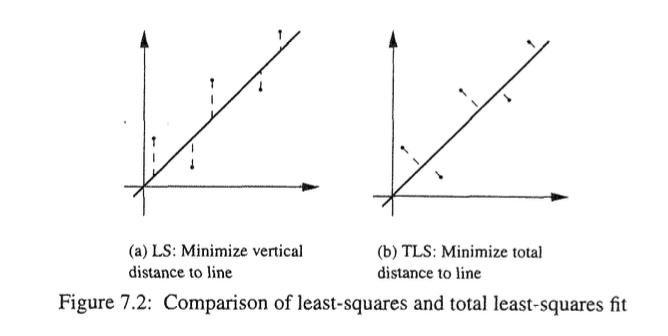
\includegraphics[width=0.75\linewidth]{img/tlsvsls.png}
    
    
\end{figure}

\subsection{Kaczmarz Algorithm}
The Kaczmarz algorithm, also known as the Algebraic Reconstruction Technique (ART) in some contexts, is an iterative method for solving linear systems of equations. Its particular strength is in solving overdetermined systems, which are systems with more equations than unknowns.\\

The algorithm iteratively projects a solution estimate onto the solution set of each equation, one at a time, and repeats this process until convergence to a close-enough solution of linear equations \( A\mathbf{x} = \mathbf{b} \). The procedure is as follows:

\begin{enumerate}
    \item Initialise with any vector \( \mathbf{x}_0 \in \mathbb{R}^n \).
    \item For \( k = 1, 2, \dots, \text{iter} \):
    \begin{itemize}
        \item Compute the next estimate \( \mathbf{x}_{k+1} \) by projecting \( \mathbf{x}_k \) onto the hyperplane defined by the \( i \)-th equation, where \( i = k \mod m + 1 \):
        \[ \mathbf{x}_{k+1} = \mathbf{x}_k + \frac{b_i - \mathbf{a}_i^T \mathbf{x}_k}{\|\mathbf{a}_i\|^2} \mathbf{a}_i \]
    \end{itemize}
    \item Repeat until convergence.
\end{enumerate}

Here, \( \mathbf{a}_i^T \) is the transpose of the \( i \)-th row of matrix \( A \) and represents a hyperplane in \( n \)-dimensional space. The term \( \frac{b_i - \mathbf{a}_i^T \mathbf{x}_k}{\|\mathbf{a}_i\|^2} \) computes the orthogonal projection of the residual \( \mathbf{r}_k = b_i - \mathbf{a}_i^T \mathbf{x}_k \) onto the hyperplane. This process geometrically "corrects" \( \mathbf{x}_k \) in the direction of the \( i \)-th row vector \( \mathbf{a}_i \), moving it closer to the solution with each iteration.
\subsubsection*{Analysis of the Approximation Error}
\begin{enumerate}
    \item Assume \( \bm{x}^* \) is the correct solution to \( A\bm{x} = \bm{b} \).
    \item At the \( (k+1) \)-th iteration, the approximation error is given by:
    \[ \bm{x}_{k+1} - \bm{x}^* = \bm{x}_k - \bm{x}^* + \frac{b_i - \bm{a}_i^T \bm{x}_k}{\| \bm{a}_i \|^2} \bm{a}_i \]
    where \( \bm{a}_i \) is the \( i \)-th row of \( A \), and \( b_i \) is the \( i \)-th component of \( \bm{b} \).
    \item To iterate, we replace \( b_i \) with \( \bm{a}_i^T \bm{x}^* \), obtaining:
    \[ \bm{x}_{k+1} - \bm{x}^* = \left( \bm{x}_k - \bm{x}^* \right) - \frac{\bm{a}_i \bm{a}_i^T}{\| \bm{a}_i \|^2} \left( \bm{x}_k - \bm{x}^* \right) \]
    \item The term \( \frac{\bm{a}_i \bm{a}_i^T}{\| \bm{a}_i \|^2} \left( \bm{x}_k - \bm{x}^* \right) \) represents the projection of the error \( \bm{x}_k - \bm{x}^* \) onto the direction of \( \bm{a}_i \).
    \item Removing the projection of the error along \( \bm{a}_i \) ensures that the error in the direction of \( \bm{a}_i \) is reduced, thus the method makes progress towards convergence.
    \item At each iteration, the norm of the error does not increase:
    \[ \| \bm{x}_{k+1} - \bm{x}^* \| \leq \| \bm{x}_k - \bm{x}^* \| \]
    This inequality shows that the Kaczmarz algorithm is convergent.
\end{enumerate}

\section{Summary}
\begin{table}[h]
\centering
\begin{tabular}{ | m{4cm} | m{3cm} | m{4cm} | m{4.5cm} | }
\hline
\textbf{Scenario} & \textbf{Number of exact Solutions} & \textbf{Type of Solution} & \textbf{Solution} \\
\hline
\( A \) ‘tall’ and full column rank & 0 or 1 & Least square: \( \min\limits_{\mathbf{x}} \|\mathbf{Ax} - \mathbf{b}\| \) & \( \mathbf{x}_{ls} = (A^HA)^{-1}A^H\mathbf{b} \) \\
\hline
\( A \) ‘fat’ and full row rank & Infinitely many solutions & Minimum-norm solution: \( \min\limits_{\mathbf{x}} \|\mathbf{x}\| \) subject to \( A\mathbf{x}=\mathbf{b} \) & \( \mathbf{x}_{MN} = A^H(AA^H)^{-1}\mathbf{b} \) \\
\hline
\( A \) neither full row nor full column rank & 0 or infinitely many solutions & Minimum-norm least square solution & \( \mathbf{\hat{x}} = V\mathbf{\Sigma}^+U^H\mathbf{b} \) with \( A = U\mathbf{\Sigma}V^H \) \\
\hline
\( A \) square and full rank (trivial) & 1 & Unique exact solution & \( \mathbf{x} = A^{-1}\mathbf{b} \) \\
\hline
\end{tabular}
\caption{Solutions to Linear Systems Based on Matrix Structure}
\end{table}

\begin{table}[h!]
\centering
\begin{tabular}{>{\centering\arraybackslash}m{1.5cm} >{\centering\arraybackslash}m{2cm} >{\centering\arraybackslash}m{4cm} >{\centering\arraybackslash}m{2cm} >{\centering\arraybackslash}m{2cm} >{\centering\arraybackslash}m{3cm}}
\toprule
\textbf{Form} & \textbf{Condition} & \textbf{Description} & \textbf{Inverse} & \textbf{Powers} & \textbf{Notes} \\
\midrule
\( S \Lambda S^{-1} \) & Diagonalisable & A matrix is diagonalisable if it can be expressed as the product of an invertible matrix \( S \), a diagonal matrix \( \Lambda \) containing the eigenvalues, and the inverse of \( S \). & \( S \Lambda^{-1} S^{-1} \) & \( S \Lambda^k S^{-1} \) & Suitable for square matrices with \( n \) linearly independent eigenvectors. \\
\addlinespace
\( U \Sigma V^T \) & Any matrix & SVD decomposes any matrix into the product of an orthogonal/unitary matrix \( U \), a diagonal matrix \( \Sigma \) with singular values, and the transpose (or conjugate transpose for complex matrices) of an orthogonal/unitary matrix \( V \). $A^+$ is used for matrices that are not full rank or not invertible. It provides a 'best fit' solution to a system of linear equations. & \( V \Sigma^{-1} U^T \) for invertible \( \Sigma \) (all values on diagonal nonzero) \( A^+ = V \Sigma^+ U^H \) & Generally not defined. & Applicable to all matrices, including non-square ones. When \( A \) is square and full rank, \( V^T = V^{-1} \). $\Sigma^+$ is the reciprocal of values along diagonal, and zero where values are zero. \\
% \addlinespace
% \( A=U \Sigma V^H \) & Non-invertible or rank-deficient & The pseudoinverse $A^+$ is used for matrices that are not full rank or not invertible. It provides a 'best fit' solution to a system of linear equations. & \( A^+ = V \Sigma^+ U^H \). & Not typically computed. & Applicable to any matrix, including non-square ones.  $\Sigma^+$ is the reciprocal of values along diagonal, and zero where values are zero. \\
\addlinespace
\( Q \Lambda Q^T \) & Symmetric Matrices & For symmetric matrices, they can be decomposed into the product of an orthogonal matrix \( Q \), a diagonal matrix \( \Lambda \), and the transpose of \( Q \). & \( Q \Lambda^{-1} Q^T \) & \( Q \Lambda^k Q^T \) & \( Q \) is orthogonal, hence \( Q^T = Q^{-1} \). This is the spectral decomposition. \\
% \addlinespace
% \( R^T R \) & Positive Definite & Cholesky Decomposition is for symmetric and positive definite matrices. It factors the matrix into an upper triangular matrix \( R \) and its transpose. & \( (R^T)^{-1} R^{-1} \) & \( (R^T R)^k \) & Efficient for computational purposes when dealing with positive definite matrices. \\
\addlinespace
\( PA = LU \) & LU Decomposition & The matrix \( A \) is decomposed with the aid of a permutation matrix \( P \), to account for pivoting, into a product of a lower triangular matrix \( L \) and an upper triangular matrix \( U \). &$ A^{-1} = (LU)^{-1}P = U^{-1}L^{-1}P $  &Usually numerically computed  &  For non-integer and negative powers, typically, the LU decomposition is not used; instead, eigenvalue decomposition or other numerical methods are more suitable.\\

\addlinespace
% \( PDP^{-1} \) or \( PDP^* \) & Complex Matrices & For complex matrices that are diagonalisable, they can be decomposed into the product of a matrix \( P \), a diagonal matrix \( D \), and the inverse (or conjugate transpose) of \( P \). & \( PD^{-1}P^{-1} \) or \( PD^{-1}P^* \) & \( PD^kP^{-1} \) or \( PD^kP^* \) & If the matrix is Hermitian (equal to its conjugate transpose), \( P \) is unitary and the decomposition is a form of spectral decomposition. \\
\bottomrule
\end{tabular}
\caption{Matrix Representations and Their Properties}
\label{table:matrix_representations}
\end{table}
